\section{Empirical Demonstration}

We demonstrate the framework on a graph routing problem. The goal is not to evaluate routing algorithms, but to show how the decision-valued map makes representational dependence observable in a concrete setting.

\subsection{Setup}

\textbf{Snapshot.} We fix a directed graph with node set $V$ ($|V| = 564$), edge set $E$, and immutable edge attributes including baseline costs derived from geographic distance and a normalized stress metric. The snapshot is content-addressed and frozen before any engine execution. We fix a single origin-destination query: start node 85, end node 50.

\textbf{Representation family.} Each representation encodes the graph's edge costs as a deterministic function of the frozen edge attributes. Two representation parameters control the cost surface: \texttt{neighbor\_weight}, a weight applied to a neighbor-based cost component (tested at 0.5 and 1.0), and \texttt{second\_order\_weight}, a weight applied to a second-order cost component (tested at 0.25 and 0.5). Each sweep varies one parameter while holding the other fixed, producing two representation variants per sweep and four engine evaluations total.

\textbf{Engine.} A fixed shortest-path solver (Dijkstra's algorithm~\cite{dijkstra1959note}), with configuration and version held constant across all runs. Execution times ranged from 0.5 to 1.4 milliseconds.

\textbf{Equivalence policy.} Policy \texttt{pol\_d8da\-3e00\-e958\-4eb1} (version 1.0.0): exact match on the canonicalized node sequence of the computed route. Two routes are assigned the same decision identity if and only if they traverse identical node sequences. The policy uses SHA-256 over JSON-serialized, sorted-key, UTF-8-encoded route nodes.

\subsection{Results: Identity Persistence and Boundary Formation}

\textbf{Neighbor weight sweep} (0.5 $\to$ 1.0, second-order weight fixed at 0.25). Both representations yield the same route:

\smallskip
\noindent\textit{Decision A:} $[85, 176, 463, 14, 404, 76, 406, 407, 223, 200, 311, 310, 314, 322, 323, 50]$ \\ (16 nodes, decision identifier \texttt{dec\_e280\ldots}).

\smallskip
\noindent Doubling the neighbor weight from 0.5 to 1.0 does not change route identity. This parameter range constitutes a persistence region under the tested policy (Figure~\ref{fig:persistence}).

\textbf{Second-order weight sweep} (0.25 $\to$ 0.5, neighbor weight fixed at 0.5). The two representations yield different routes:

\smallskip
\noindent\textit{Decision A} (second-order weight = 0.25): same route as above.

\noindent\textit{Decision B} (second-order weight = 0.5): $[85, 411, 419, 422, 332, 204, 500, 369, 79, 402, 473, 502, 501, 50]$ \\ (14 nodes, decision identifier \texttt{dec\_c2dd\ldots}).

\smallskip
\noindent The route changes entirely: a different sequence of 14 nodes instead of 16, traversing a different region of the graph. The boundary between these two decision identities lies between second-order weight values 0.25 and 0.5 (Figure~\ref{fig:boundary}). This is a fracture: a small parameter change induces a qualitative change in the discrete outcome.

\begin{figure}[t]
  \centering
  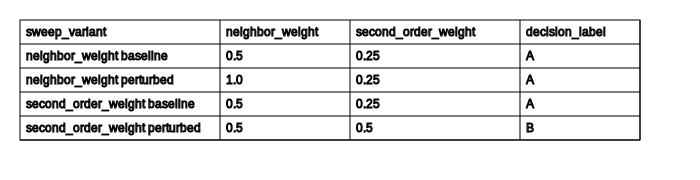
\includegraphics[width=\linewidth]{figures/figure2_primary_sweep.pdf}
  \caption{Primary representational sweep. Each column corresponds to a representation variant defined by its weight parameter setting. Decision identity (A or B) is assigned by the equivalence policy based on the route node sequence. The neighbor weight sweep (left) shows identity persistence; the second-order weight sweep (right) shows a boundary.}
  \label{fig:primary-sweep}
\end{figure}

\begin{figure}[t]
  \centering
  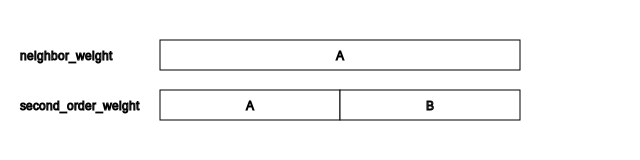
\includegraphics[width=\linewidth]{figures/figure3_identity_persistence.pdf}
  \caption{Identity persistence regions derived from the sweep in Figure~\ref{fig:primary-sweep}. The neighbor weight parameter spans a single persistence region (Decision~A). The second-order weight parameter spans two regions (A and B) separated by a boundary between 0.25 and 0.5.}
  \label{fig:persistence}
\end{figure}

\begin{figure}[t]
  \centering
  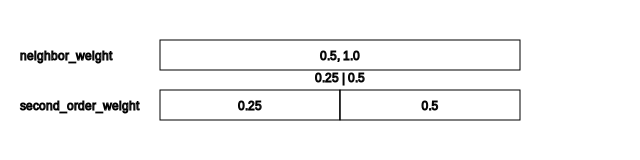
\includegraphics[width=\linewidth]{figures/figure4_boundary_fracture.pdf}
  \caption{Boundary and fracture localization. The neighbor weight sweep shows no boundary (\texttt{route\_changed = false}). The second-order weight sweep shows a boundary between 0.25 and 0.5 (\texttt{route\_changed = true}, \texttt{edge\_order\_changed = true}).}
  \label{fig:boundary}
\end{figure}

Table~\ref{tab:sweep-summary} summarizes the sweep results.

\begin{table}[t]
\centering
\caption{Summary of representational sweep results.}
\label{tab:sweep-summary}
\smallskip
\tablestyle
\rowcolors{2}{tableShade}{white}
\begin{tabular}{@{\hskip 8pt}l l c c l@{\hskip 8pt}}
\toprule
\rowcolor{white}
\textbf{Sweep parameter} & \textbf{Value} & \textbf{Decision} & \textbf{Nodes} & \textbf{Boundary?} \\
\midrule
\texttt{neighbor\_weight} & 0.5 & A & 16 & \\
\texttt{neighbor\_weight} & 1.0 & A & 16 & No \\
\texttt{second\_order\_weight} & 0.25 & A & 16 & \\
\texttt{second\_order\_weight} & 0.5 & B & 14 & Yes \\
\bottomrule
\end{tabular}
\end{table}

\subsection{Replay Verification}

We verify replay determinism for a decision produced by the sweep. The replay procedure loads the stored raw output from its persisted URI, recomputes the equivalence policy identifier, extracts the decision payload, and recomputes both the payload hash and the decision identifier.

All recomputed values match the persisted values exactly (Table~\ref{tab:replay}, Figure~\ref{fig:replay}):

\begin{table}[ht]
\centering
\caption{Replay verification results for decision \texttt{dec\_e280\ldots}.}
\label{tab:replay}
\smallskip
\tablestyle
\rowcolors{2}{tableShade}{white}
\begin{tabular}{@{\hskip 8pt}l l l@{\hskip 8pt}}
\toprule
\rowcolor{white}
\textbf{Field} & \textbf{Persisted} & \textbf{Recomputed} \\
\midrule
Policy ID & \texttt{pol\_d8da3e00e9584eb1} & \texttt{pol\_d8da3e00e9584eb1} \\
Payload hash & \texttt{3a9d63ac28378116} & \texttt{3a9d63ac28378116} \\
Decision ID & \texttt{dec\_e28092c4dc33b8f1} & \texttt{dec\_e28092c4dc33b8f1} \\
\bottomrule
\end{tabular}
\end{table}

The replay writes no new rows and modifies no database state. Table counts before and after replay are identical (1 engine run, 1 decision, 1 f\_map entry). This confirms that the content-addressing chain from raw output through policy application to decision identity is deterministic and end-to-end auditable.

\begin{figure}[t]
  \centering
  \begin{tikzpicture}[
    node distance=5mm and 8mm,
    box/.style={draw, rounded corners, align=center, inner sep=5pt, text width=30mm, font=\small},
    artifact/.style={box, fill=tableShade},
    result/.style={box, fill=black!8, font=\small\sffamily},
    arrow/.style={-Latex, thick},
    eq/.style={font=\small\sffamily, text=black!60}
  ]
  % Left column: persisted
  \node[font=\small\bfseries\sffamily] (plabel) {Persisted};
  \node[artifact, below=6mm of plabel] (ppol) {\texttt{pol\_d8da\ldots}\\{\scriptsize policy ID}};
  \node[artifact, below=of ppol] (phash) {\texttt{3a9d63ac\ldots}\\{\scriptsize payload hash}};
  \node[artifact, below=of phash] (pdec) {\texttt{dec\_e280\ldots}\\{\scriptsize decision ID}};

  % Right column: recomputed
  \node[font=\small\bfseries\sffamily, right=22mm of plabel] (rlabel) {Recomputed};
  \node[artifact, below=6mm of rlabel] (rpol) {\texttt{pol\_d8da\ldots}\\{\scriptsize policy ID}};
  \node[artifact, below=of rpol] (rhash) {\texttt{3a9d63ac\ldots}\\{\scriptsize payload hash}};
  \node[artifact, below=of rhash] (rdec) {\texttt{dec\_e280\ldots}\\{\scriptsize decision ID}};

  % Equality checks
  \draw[thick, black!40] (ppol.east) -- node[eq, above] {$=$} (rpol.west);
  \draw[thick, black!40] (phash.east) -- node[eq, above] {$=$} (rhash.west);
  \draw[thick, black!40] (pdec.east) -- node[eq, above] {$=$} (rdec.west);

  % Source arrow
  \node[box, left=12mm of ppol, text width=22mm] (raw) {Raw output\\{\scriptsize stored artifact}};
  \draw[arrow] (raw.east) -- (ppol.west);

  % Recompute arrow
  \node[box, right=12mm of rpol, text width=22mm] (engine) {Recompute\\{\scriptsize from artifact}};
  \draw[arrow] (engine.west) -- (rpol.east);

  % Verdict
  \node[result, below=10mm of $(pdec.south)!0.5!(rdec.south)$, text width=22mm, line width=0.8pt] (verdict) {\textbf{PASS}\\{\scriptsize 0 rows written}};
  \draw[arrow] (pdec.south) |- (verdict.west);
  \draw[arrow] (rdec.south) |- (verdict.east);

  \end{tikzpicture}
  \caption{Replay verification. Persisted identifiers (left) are compared against values recomputed from stored artifacts (right). All three fields match exactly. No rows are written and no database state is modified.}
  \label{fig:replay}
\end{figure}
